\chapter{粒子物理}\label{ch:b3:particle-physics}

% Provenance (not for print): second half of the "physique subatomique"
% module common to the surveyed third-year curricula: standard model
% inventory, interactions, conservation laws, detectors.

逐层剥去物质的结构——分子、原子、
原子核、核子——剥离戛然而止于一份简短的清单：
六种\emph{夸克}、六种\emph{轻子}、若干种力的载体，
以及 2012 年发现的那个腼腆的标量粒子。你曾接触过的一切物质，
全都只是这份清单上的三个条目；其余粒子曾存在于宇宙
诞生后的最初一微秒，并会在任何
$E = mc^2$ 得以充分兑现之处短暂重现——宇宙射线碰撞与加速器
环。本章盘点这些内容：粒子、四种
推动它们运动的相互作用、守恒定律，
（\cref{ch:b3:lagrangian-mechanics}中的诺特流，如今用于亚原子尺度
的守恒核算），以及记录这一切的探测器。本章结尾
回到你自家的阁楼，数一数十公里高空中产生的μ子。

\section{粒子清单}

\begin{definition}[轻子、夸克、强子]\label{def:b3:particle-physics:zoo}
\index{轻子}\index{夸克}\index{强子}\index{重子}\index{介子}\index{反粒子}
物质的基本组成单元是自旋为 $\tfrac12$ 的费米子
（见\cref{ch:b3:spin-two-level}、\cref{ch:b3:identical-particles}），
分为两族，每族六种。\emph{轻子}不感受强相互作用：
电子、μ子和τ子（电荷 $-e$，质量依次增大），
以及它们的三种中微子——质量近乎为零，
几乎无法探测。\emph{夸克}有六种味：上、下、
奇、粲、底、顶，电荷分别为 $+\tfrac23e$（u、c、
t）和 $-\tfrac13e$（d、s、b），且从不单独被观测到：
\emph{禁闭}将它们束缚为\emph{强子}——三夸克
\emph{重子}（质子 $=$ uud，中子 $=$ udd）以及
夸克–反夸克\emph{介子}（π 介子、K 介子）。每种粒子都有一个
质量相同、电荷相反的\emph{反粒子}
（见\cref{exo:b3:particle-physics:8}）。普通物质只用到
第一代粒子——u、d、e、$\nu_{\text{e}}$；较重的另外两代
据目前所知，二者仅质量不同。物理学至今仍在追问：
“谁点了这道菜？”
\end{definition}

\begin{omfigure}
\begin{tikzpicture}[scale=0.98,
  cell/.style={draw, minimum width=1.28cm, minimum height=1.05cm,
    font=\scriptsize, align=center, inner sep=1pt}]
  % quarks (2x3)
  \foreach \i/\n/\m in {0/u/{$+\tfrac23$}, 1/c/{$+\tfrac23$}, 2/t/{$+\tfrac23$}}
    \node[cell, fill=omDef!18] at (1.4*\i,1.1) {\textbf{\n}\\\m};
  \foreach \i/\n/\m in {0/d/{$-\tfrac13$}, 1/s/{$-\tfrac13$}, 2/b/{$-\tfrac13$}}
    \node[cell, fill=omDef!18] at (1.4*\i,0) {\textbf{\n}\\\m};
  % leptons
  \foreach \i/\n in {0/{e}, 1/{$\mu$}, 2/{$\tau$}}
    \node[cell, fill=omExo!20] at (1.4*\i,-1.35) {\textbf{\n}\\$-1$};
  \foreach \i/\n in {0/{$\nu_{\text{e}}$}, 1/{$\nu_\mu$}, 2/{$\nu_\tau$}}
    \node[cell, fill=omExo!20] at (1.4*\i,-2.45) {\textbf{\n}\\$0$};
  % bosons
  \node[cell, fill=omThm!15] at (5.0,1.1) {\textbf{g}\\强};
  \node[cell, fill=omThm!15] at (5.0,0) {\textbf{$\gamma$}\\电磁};
  \node[cell, fill=omThm!15] at (5.0,-1.35) {\textbf{W, Z}\\弱};
  \node[cell, fill=omThm!15] at (6.5,1.1) {\textbf{H}\\希格斯};
  % generation labels
  \node[font=\scriptsize, anchor=south] at (0,1.75) {第一代};
  \node[font=\scriptsize, anchor=south] at (1.4,1.75) {第二代};
  \node[font=\scriptsize, anchor=south] at (2.8,1.75) {第三代};
  \node[font=\scriptsize, anchor=south] at (5.75,1.75) {载体};
  \node[font=\scriptsize, rotate=90, anchor=south] at (-1.05,0.55) {夸克};
  \node[font=\scriptsize, rotate=90, anchor=south] at (-1.05,-1.9) {轻子};
\end{tikzpicture}

{\small 标准模型粒子表（电荷以 $e$ 为单位）。其中一列
构成了一切原子；另外两列只是
代价高昂的回响。引力在这些质量尺度下弱得无法测量，在此表中没有
一席之地——这是该模型最著名的空缺。}
\end{omfigure}

\begin{remark}[四种相互作用]\label{rem:b3:particle-physics:forces}
\index{强相互作用}\index{弱相互作用}\index{电弱相互作用}
每个过程都是四种相互作用之一在起作用，每种相互作用都由各自的
玻色子传递。\emph{强相互作用}（胶子）以一种
随距离\emph{增大}的势能束缚夸克：把两个夸克拉开，
被拉长的场便会断裂，生成一对新的夸克–反夸克
（见\cref{exo:b3:particle-physics:1}）。由此产生禁闭，
其残余则将原子核粘合在一起
（见\cref{ch:b3:nuclear-physics}）。\emph{电磁相互作用}（光子，
质量为零，作用范围无限）支配着化学与光。
\emph{弱}相互作用（W 与 Z 玻色子，质量很大，约为
$\approx80$--$\qty{91}{GeV}$，作用范围 $10^{-3}\,\unit{fm}$，
故称“弱”），是唯一能改变味的相互作用——$\beta$ 衰变
是一个 d 夸克变成 u 夸克
（见\cref{prop:b3:particle-physics:conservation}），也是
中微子唯一响应的相互作用。\emph{引力}比两质子之间的
电磁相互作用弱 $10^{36}$ 倍，在实验室中毫无
作用——然而引力不受屏蔽、作用长程，它将贯穿
\cref{ch:b3:astrophysics}的全部内容。电磁相互作用与弱
相互作用在高能下统一为单一的\emph{电弱相互作用}，
——在我们所处的低能下，由希格斯
场的对称性破缺将二者分开（见\cref{exo:b3:particle-physics:9}）。
\end{remark}

\section{核算：守恒定律}

\begin{proposition}[粒子反应的守恒定律]\label{prop:b3:particle-physics:conservation}
\index{重子数}\index{轻子数}\index{守恒定律!粒子}
一个反应只有在“账目”平衡时才能发生。总是守恒的量有
能量–动量
（见\cref{ch:b3:relativistic-dynamics}）、角动量和
电荷——诺特定理
（见\cref{thm:b3:lagrangian-mechanics:noether}）为每一项提供依据。
迄今所有观测到的反应中都守恒的量：\emph{重子数}
$B$（重子 $+1$，反重子 $-1$）和\emph{轻子数}
$L$（按每一代计，精度极高）。因此质子是最轻的
重子，没有任何衰变途径——物质的稳定性
是一条核算定理，而 $\beta$ 衰变必须放出
一个反中微子：
\[
\text{n} \;\to\; \text{p} + \text{e}^- + \bar\nu_{\text{e}}
\qquad (\text{夸克层次： } \text{d} \to \text{u} +
\text{e}^- + \bar\nu_{\text{e}}) ,
\]
这样便守恒了 $L$（并解释了电子能量的连续
能谱——这几乎让物理学丧失对能量守恒的信念，
直到泡利提出中微子将其挽救）。
味（奇异数、粲数）在强相互作用和
电磁过程中守恒，但\emph{被弱相互作用破坏}：奇异粒子
成对大量产生，随后缓慢而单独地衰变——
$10^{13}$ 倍的差距，位于 $\qty{e-23}{s}$ 的强衰变寿命
与 $\qty{e-10}{s}$ 的弱衰变寿命之间，正是
判定衰变由哪种力所主导的标志。
\end{proposition}
\admitted

\begin{omfigure}
\begin{tikzpicture}[scale=1.0]
  % neutron -> proton beta decay quark diagram
  % three quark lines left to right
  \draw[omDef, thick] (0,2.0) -- (7.2,2.0);
  \draw[omDef, thick] (0,1.45) -- (7.2,1.45);
  \draw[omDef, thick] (0,0.9) -- (3.3,0.9);
  \draw[omThm, thick] (3.3,0.9) -- (7.2,0.9);
  \node[omDef, font=\scriptsize, anchor=east] at (-0.1,2.0) {u};
  \node[omDef, font=\scriptsize, anchor=east] at (-0.1,1.45) {d};
  \node[omDef, font=\scriptsize, anchor=east] at (-0.1,0.9) {d};
  \node[omThm, font=\scriptsize, anchor=west] at (7.3,0.9) {u};
  \node[font=\scriptsize, anchor=west] at (7.3,1.45) {d};
  \node[font=\scriptsize, anchor=west] at (7.3,2.0) {u};
  % W boson wavy-ish (zigzag)
  \draw[omExo, thick] (3.3,0.9)
    -- (3.75,0.55) -- (4.05,0.75) -- (4.35,0.35) -- (4.65,0.55)
    -- (4.95,0.15) -- (5.25,0.35) -- (5.55,-0.05);
  \node[omExo, font=\scriptsize, anchor=west] at (4.75,0.72) {W$^-$};
  % electron and antineutrino
  \draw[thick] (5.55,-0.05) -- (7.2,0.25);
  \draw[thick] (5.55,-0.05) -- (7.2,-0.55);
  \node[font=\scriptsize, anchor=west] at (7.3,0.25) {e$^-$};
  \node[font=\scriptsize, anchor=west] at (7.3,-0.55) {$\bar\nu_{\text{e}}$};
  % braces labels
  \node[font=\scriptsize, anchor=east] at (-0.75,1.45) {中子};
  \node[font=\scriptsize, anchor=west] at (8.35,1.45) {质子};
\end{tikzpicture}

{\small $\beta$ 衰变，放大到夸克层次：一个 d 夸克
通过发射一个虚的 W$^-$ 变为 u 夸克，它随即物化为
电子加反中微子。各项守恒：电荷
$-\tfrac13 = +\tfrac23 - 1 + 0$，重子数，轻子数。}
\end{omfigure}

\section{粒子的制造与观测}

\begin{remark}[加速器与探测器]\label{rem:b3:particle-physics:machines}
\index{对撞机}\index{粒子探测器}
加速粒子有两个理由：\emph{分辨率}——探针看不到
比其波长 $\lambda = h/p$ 更精细的细节（在
\cref{ch:b3:crystalline-solids}中用的是埃，飞米则
需要 \unit{GeV} 量级的能量）——以及\emph{产生}：碰撞能量
转化为新的质量，两束粒子迎头对撞时能把它全部用上
（固定靶则大部分能量都用于让碎片向前运动：
见\cref{exo:b3:particle-physics:4}）。环形对撞机让同一批粒子
反复穿过同一个加速间隙，同时
磁铁负责引导它们——代价是同步辐射，
其大小 $\propto\gamma^4$，这正是发现希格斯玻色子的那台环形装置
对撞的是重质子，而非轻如鸿毛的电子。对撞点周围
排列着洋葱式的分层探测器，每层回答一个问题：
\emph{径迹室}借磁场使带电粒子径迹弯曲（测动量）；
电磁\emph{量能器}吸收电子和
光子（测能量）；强子量能器则吸收 π 介子和质子；
只有 μ 子能穿透到最外层的探测室——
依靠穿透深度的差异来鉴别粒子。中微子则以丢失动量的形式离开：
靠守恒量的核算来探测那些什么也拦不住的粒子。
\end{remark}

\begin{omfigure}
\begin{tikzpicture}[scale=1.0]
  % quadrant onion detector
  \fill[omDef!10] (0,0) -- (4.7,0) arc (0:80:4.7) -- cycle;
  \fill[omExo!18] (0,0) -- (3.5,0) arc (0:80:3.5) -- cycle;
  \fill[omThm!12] (0,0) -- (2.3,0) arc (0:80:2.3) -- cycle;
  \fill[white] (0,0) -- (1.2,0) arc (0:80:1.2) -- cycle;
  \foreach \r in {1.2,2.3,3.5,4.7} \draw[gray] (\r,0) arc (0:80:\r);
  \draw[gray] (0,0) -- (4.7,0);
  \draw[gray] (0,0) -- (80:4.7);
  % labels of layers, along the free bottom edge
  \node[font=\tiny, anchor=north] at (1.75,-0.12) {径迹室};
  \node[font=\tiny, anchor=north] at (2.9,-0.12) {电磁量能器};
  \node[font=\tiny, anchor=north] at (4.1,-0.12) {强子量能器};
  \node[font=\tiny, anchor=west] at (12:4.85) {μ 子探测室};
  % particle tracks from origin
  % electron: curved, stops in ecal
  \draw[omDef, thick] (0,0) .. controls (1.1,0.62) .. (2.05,1.55);
  \fill[omDef] (2.6,1.9) circle (2pt);
  \node[omDef, font=\tiny, anchor=south west] at (2.5,1.98) {e$^-$};
  % photon: straight dashed (neutral), stops in ecal
  \draw[omDef, dashed] (0,0) -- (55:2.75);
  \fill[omDef] (55:2.95) circle (2pt);
  \node[omDef, font=\tiny, anchor=south] at (55:3.2) {$\gamma$};
  % pion: curved into hadronic
  \draw[omThm, thick] (0,0) .. controls (0.75:2.0) and (5:2.6) .. (12:3.9);
  \fill[omThm] (14:4.1) circle (2pt);
  \node[omThm, font=\tiny, anchor=north] at (10:4.28) {$\pi$};
  % muon: nearly straight, exits
  \draw[omExo, very thick] (0,0) .. controls (70:2.4) .. (73:5.2);
  \node[omExo, font=\tiny, anchor=south] at (73:5.35) {$\mu$};
\end{tikzpicture}

{\small 对撞机探测器的截面图。每种粒子都留下各自的特征：
带电径迹在径迹室的磁场中弯曲；
电子和光子在内层量能器中被吸收，
强子在外层量能器中被吸收；只有 μ 子能到达最远的探测室；而
那些未被探测到的粒子——中微子——则由丢失的
动量推断得出。}
\end{omfigure}

\begin{remark}[希格斯与未竟之账]\label{rem:b3:particle-physics:higgs}
\index{希格斯玻色子}\index{暗物质}
标准模型的对称性禁止其粒子具有裸质量；
\emph{希格斯场}充满全空间，并具有非零凝聚——
即\cref{ch:b3:phase-transitions}中的双势阱选择，
只是把它提升到了真空本身，
——打破了对称性，并通过耦合赋予粒子质量：
粒子越重，耦合越强。它自身的量子，即希格斯
玻色子（\qty{125}{GeV}，2012 年发现）补全了这张表。
未竟之账还更长：中微子在不同的味之间振荡，
因而必须具有模型从未写入的质量
（见\cref{exo:b3:particle-physics:10}）；星系的旋转仿佛被
比发光物质多五倍的物质束缚着；
（见\cref{ch:b3:astrophysics}）；宇宙中含有物质，
却几乎没有反物质，这一不对称性是模型中微小的
CP 破坏尚无法解释。这份清单就是
接下来一切内容的大纲。
\end{remark}

\begin{omfigure}
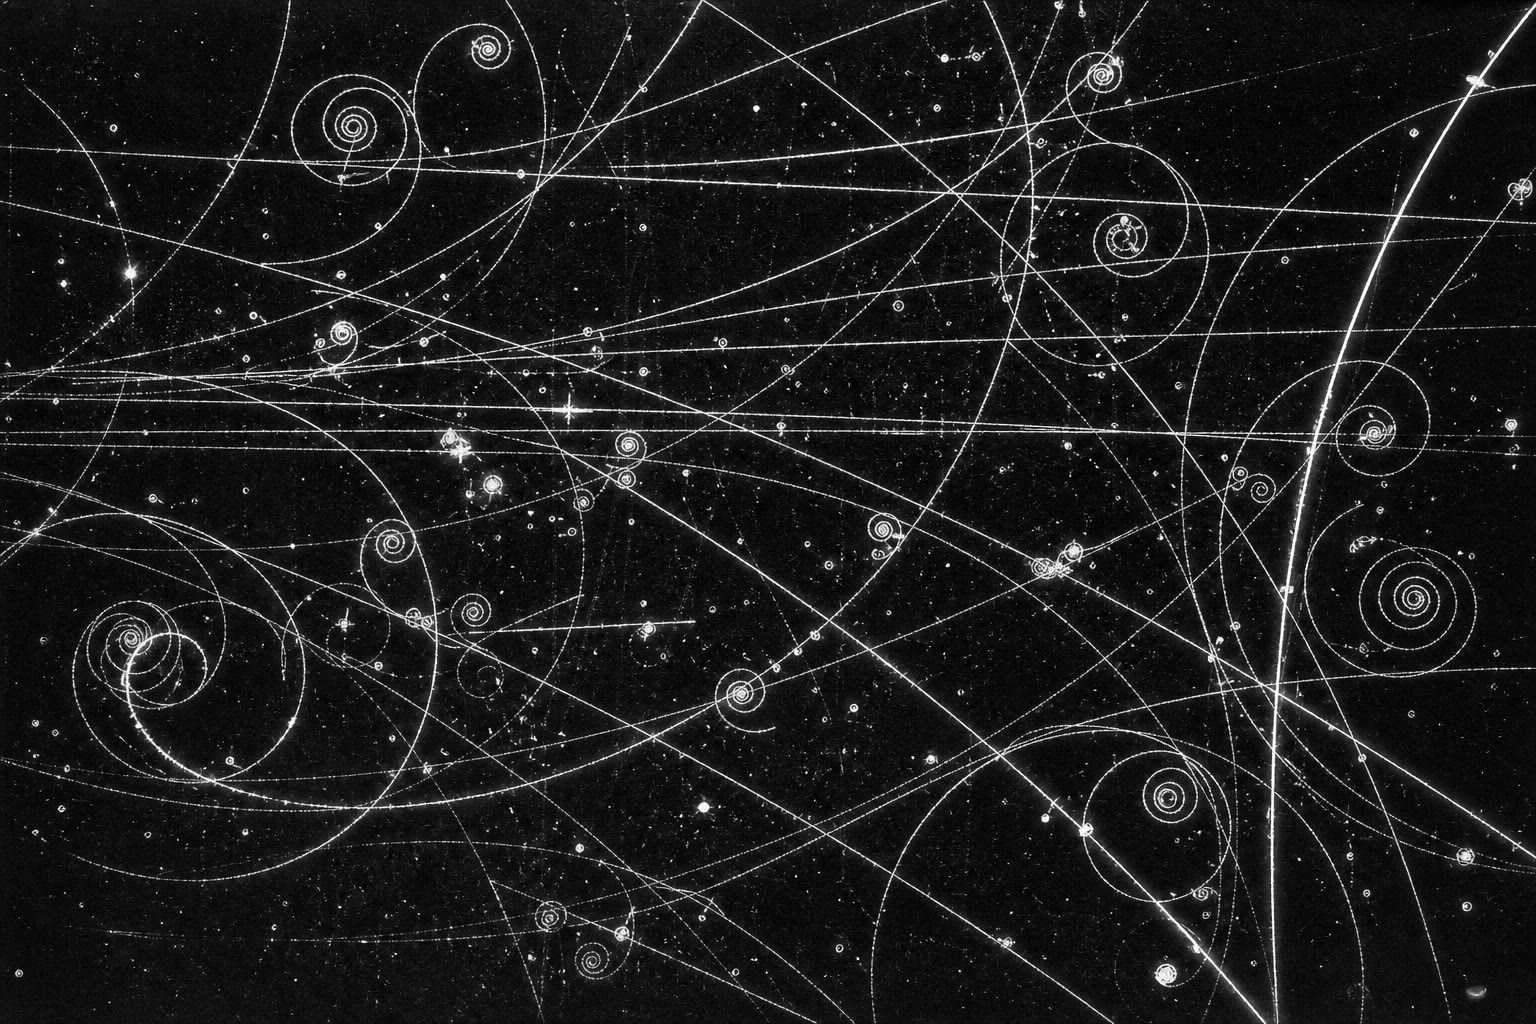
\includegraphics[width=0.58\linewidth]{images/book5/ai/b5-22-bubble-chamber-spirals.jpg}

{\small 气泡室图像：带电径迹在磁场中弯曲，电子与正电子随能量损失而沿相反方向螺旋运动。几十年来，粒子物理正是这样从此类底片上逐帧读取信息的。}
\end{omfigure}

\section{练习}

\begin{exercise}[$\star$]\label{exo:b3:particle-physics:1}
夸克运算。(a) 验证质子 p $=$ uud 与
中子 n $=$ udd 的电荷。(b) π 介子 $\pi^+$ 为 $\text{u}\bar{\text{d}}$：
请核对其电荷。(c) 试给出 $\pi^-$ 与
$\Delta^{++}$（电荷 $+2e$）的夸克组成。(d) 为何把夸克从质子中拉出时
会产生介子簇射，而非自由夸克？
\end{exercise}

\begin{exercise}[$\star$]\label{exo:b3:particle-physics:2}
分类。对以下每一种粒子：e$^-$、$\nu_\mu$、$\pi^+$、p、n、
$\mu^-$：(a) 属于轻子、重子还是介子？(b) 哪些
受强相互作用？(c) 哪些粒子单独存在时是稳定的？(d) 哪些
不会被磁场偏转？
\end{exercise}

\begin{exercise}[$\star$]\label{exo:b3:particle-physics:3}
允许还是禁止？判断下列过程，若被禁止，指出所违反的定律：
(a) $\text{n} \to \text{p} + \text{e}^- + \bar\nu_{\text{e}}$；
(b) $\text{p} \to \text{n} + \text{e}^+ + \nu_{\text{e}}$（对
\emph{自由}质子）；
(c) $\text{p} \to \text{e}^+ + \gamma$；
(d) $\mu^- \to \text{e}^- + \gamma$。
\end{exercise}

\begin{exercise}[$\star$]\label{exo:b3:particle-physics:4}
产生的代价。在氢靶上用质子束产生质子–反质子对，
需要（由
\cref{ch:b3:relativistic-dynamics}的不变质量论证）束流动能为
$6m_{\text{p}}c^2$。(a) 以 GeV 为单位求值。
(b) 在对撞机中，两束粒子各需多大动能，
方可产生同样的粒子对？(c) 计算“浪费”的比例，并说明
固定靶的能量流向何处。(d) 为何 1955 年发现反质子所用的加速器
需要 $\sim\qty{6}{GeV}$？
\end{exercise}

\begin{exercise}[$\star\star$]\label{exo:b3:particle-physics:5}
μ 子两重考察。μ 子（$m = \qty{106}{MeV}$，
$\tau = \qty{2.2}{\micro s}$）是电子的重“孪生兄弟”。(a)
$c\tau$ 对应多大距离？(b) 宇宙线 μ 子
在 \qty{15}{km} 高处产生并到达地面：存活需要多大的 $\gamma$，
对应多大能量？(c) 试从
μ 子自身的参考系描述同样的存活。(d) 为何 μ 子衰变为电子而从不衰变为质子，
又按粒子标准，其衰变为何如此
\emph{缓慢}？
\end{exercise}

\begin{exercise}[$\star\star$]\label{exo:b3:particle-physics:6}
$\beta$ 衰变的内部过程。(a) 在夸克层次写出中子衰变，
并检验所有守恒量。(b) 所发射
电子的能谱连续，直至某一端点：
试解释这曾如何威胁能量守恒，以及
泡利的中微子如何挽救了它。(c) W 玻色子的质量为
\qty{80.4}{GeV}：估算弱相互作用的
作用范围 $\hbar/m_{\text{W}}c$（$\hbar c = \qty{197}{MeV.fm}$）。(d) 利用
该作用范围，用一句话解释为何“弱”相互作用
在低能时很弱，在高能时却达到电弱统一的强度。
\end{exercise}

\begin{exercise}[$\star\star$]\label{exo:b3:particle-physics:7}
奇异量的核算。K 介子与 $\Lambda$ 超子携带一种
味，即\emph{奇异性}，强相互作用守恒而
弱相互作用则不然。(a) 解释为何宇宙线碰撞只成对产生
奇异粒子。(b) $\Lambda$ 的寿命为
$\qty{2.6e-10}{s}$——与强衰变的 $\qty{e-23}{s}$ 相比，
并判断由哪种相互作用使其衰变。(c) 两者的时间尺度之比，
以及它与日常生活中哪一比值相当，
（一秒对照什么）？(d) 这种
“奇异”行为——大量产生、迟迟不衰变——
如何迫使人们引入一个新的量子数？
\end{exercise}

\begin{exercise}[$\star\star$]\label{exo:b3:particle-physics:8}
反物质的兑现。(a) 为何
$\text{e}^+ + \text{e}^- \to \gamma$（单光子）必被禁止，
而双光子却允许？(b) 计算一克反物质与一克物质湮灭
所释放的能量，并与
\cref{exo:b3:nuclear-physics:9}中的一千克
裂变铀相比较。(c) PET 扫描仪
（\cref{exo:b3:nuclear-physics:12}）利用正电子工作：
医用正电子从何而来？(d) 制造反质子的代价，
以插座电功率计，约为其静能的 $\sim10^{6}$ 倍：
请评论反物质作为燃料。
\end{exercise}

\begin{exercise}[$\star\star\star$]\label{exo:b3:particle-physics:9}
作为相变的希格斯机制。(a) 用
\cref{exo:b3:phase-transitions:12}的语言，重述真空
位于对称性破缺势阱中意味着什么。(b) 为何 W 与 Z 获得
质量，而光子仍无质量（对称性的哪一部分得以保留）？
(c) 希格斯玻色子是场的径向振荡：在
\cref{thm:b3:phase-transitions:meanfield}的磁体中，
何者扮演这一角色？(d) 高于
$\sim10^{15}\,\unit{K}$ 时对称性恢复：宇宙
最后一次如此炽热是在何时何地（\cref{ch:b3:astrophysics}）？
\end{exercise}

\begin{exercise}[$\star\star\star$]\label{exo:b3:particle-physics:10}
数以十亿计的中微子。(a) 太阳每进行一次
$4\text{p} \to {}^4\text{He}$ 循环（\qty{26.7}{MeV}）产生两个中微子：
由太阳常数 \qty{1360}{W/m^2}，
计算地球处的中微子通量。(b) 每秒有多少个中微子穿过你的
拇指指甲（\qty{1}{cm^2}），一生中大致有多少个与你的身体
发生相互作用（取每个中微子、每米血肉的相互作用
概率为 $10^{-22}$ 量级，视为
已知）？(c) 早期
探测器只捕到预言中的三分之一的
$\nu_{\text{e}}$：说明其解决办法（振荡）及其
对标准模型的结构性后果。(d) 为何中微子探测器
要置于山下？
\end{exercise}

\begin{exercise}[$\star\star\star$]\label{exo:b3:particle-physics:11}
加速器数字。LHC 质子各自能量 $E = \qty{6.8}{TeV}$。(a)
计算 $\gamma$ 及 $1 - v/c \approx 1/2\gamma^2$。(b) 哪个
波长 $\lambda \approx hc/E$ 能探测结构，并与
质子的 \qty{0.8}{fm} 半径比较。(c) 正面碰撞
能量为 \qty{13.6}{TeV}——能产生多少个
质子静止质量？(d) 同步辐射损失正比于 $\gamma^4$：
计算固定能量下电子与质子的 $\gamma$ 之比，
并论证环形加速器宜用质子，精密
仪器宜用电子。
\end{exercise}

\begin{exercise}[$\star\star\star$]\label{exo:b3:particle-physics:12}
来自边缘的信使。有史以来记录到的最高能宇宙射线
携带 $\sim\qty{3e20}{eV}$——单个质子。(a)
换算为焦耳，并举出一个具有该动能的宏观
物体。(b) 计算其 $\gamma$，以及在其
自身参考系中银河的宽度（$\sim10^{5}$ 光年）。(c)
能量高于 $\sim\qty{5e19}{eV}$ 时，质子会与宇宙微
波背景（\cref{ch:b3:photons-phonons}）散射——
定性解释宇宙为何对它们不透明。(d) 这些
远超任何加速器的能量，为何仍
比 LHC 教给我们的更少？（考虑通量与可控性。）
\end{exercise}

\begin{omfigure}
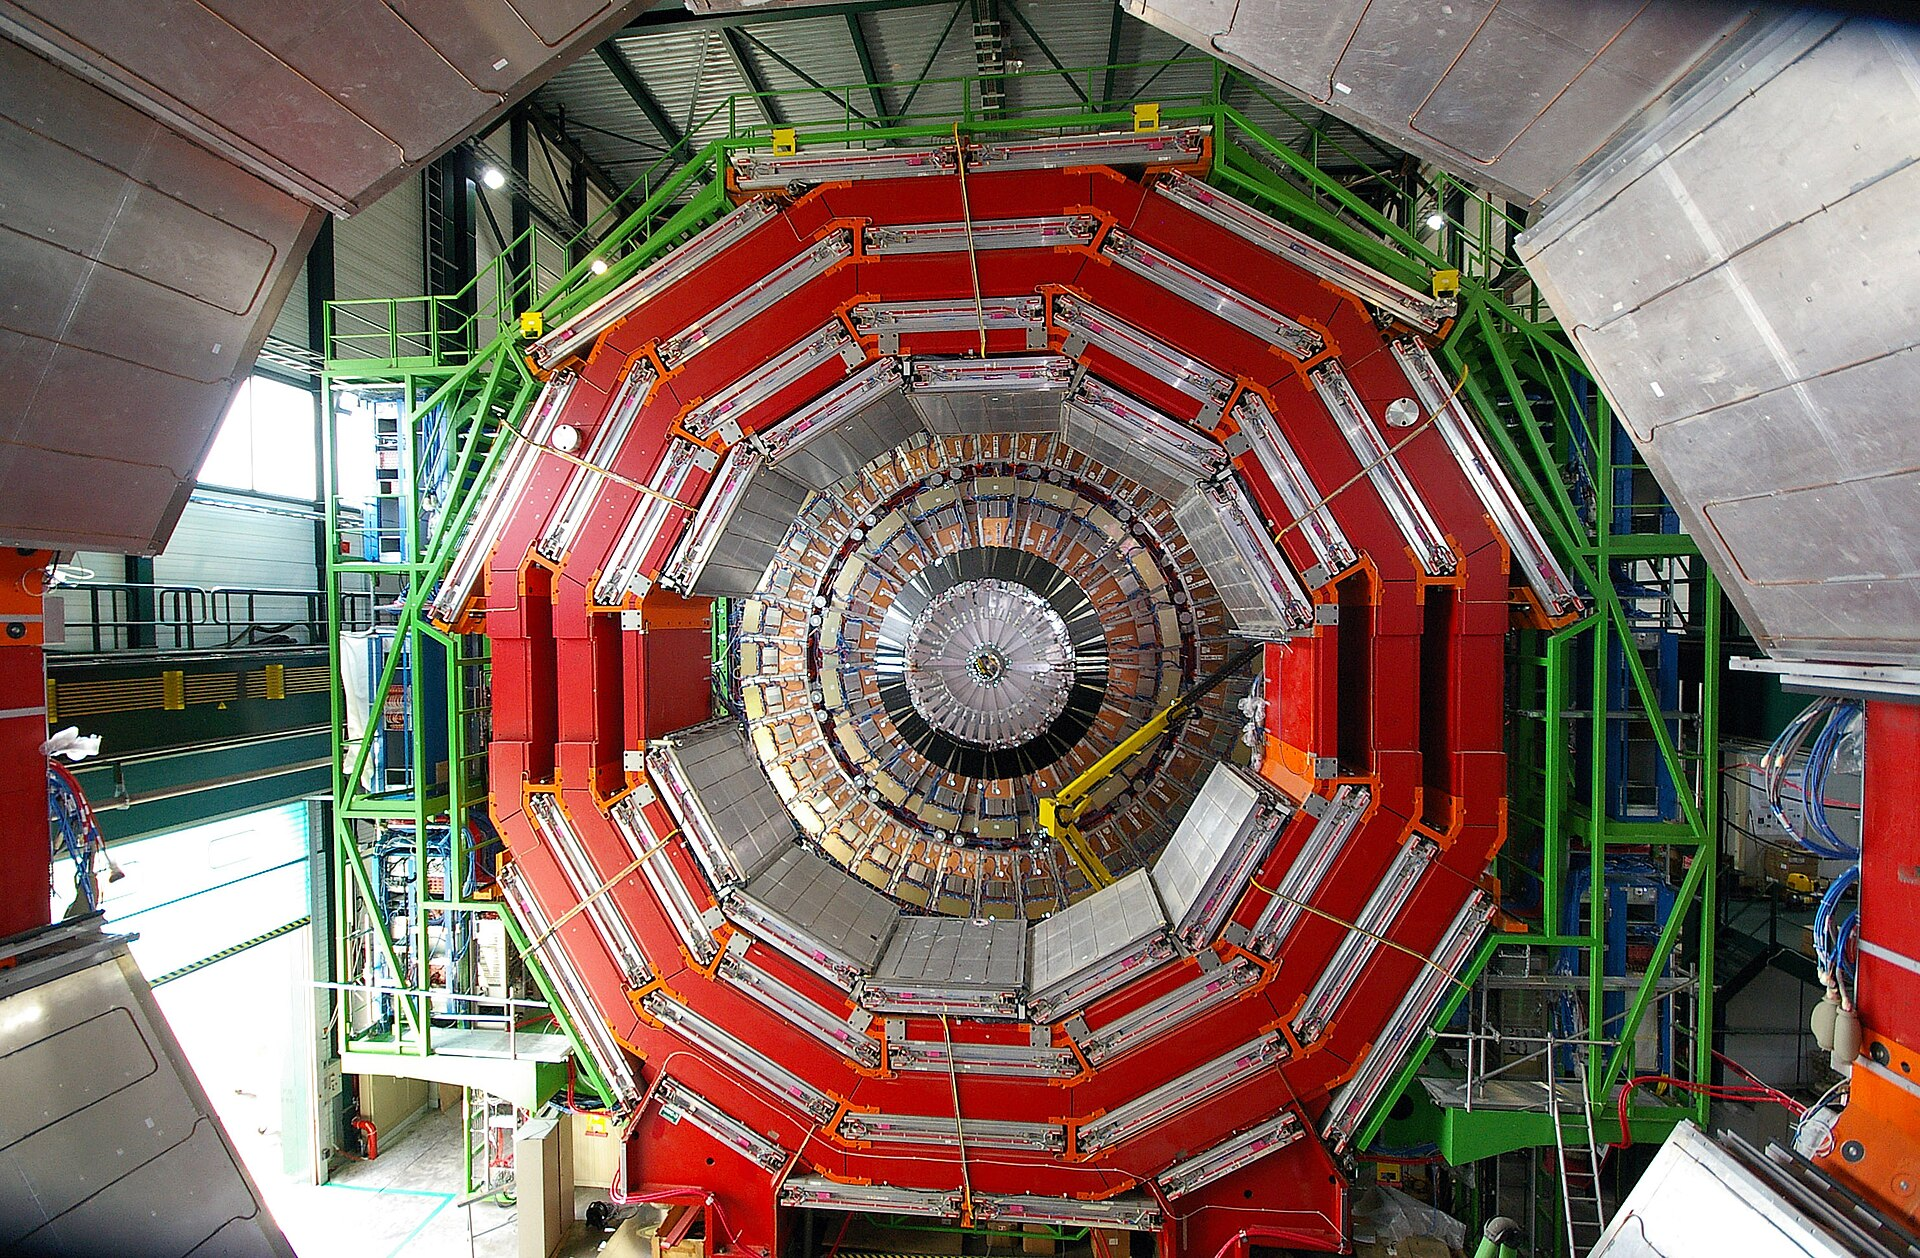
\includegraphics[width=0.62\linewidth]{images/book5/photo-cms-construction.jpg}

{\small 建造中的 CMS 探测器（照片：Julian Williams，免费使用）：桶部的洋葱层结构，正面视角，合拢前——本章末图所示原理的一万五千吨级实物。}
\end{omfigure}

\section{问题：阁楼上的 μ 子望远镜}

\begin{problem}\label{pb:b3:particle-physics:1}
\emph{阁楼上的 μ 子望远镜。}为参加科学展，你要搭建一台
宇宙射线望远镜：两块 $20\times20$\,\unit{cm} 闪烁体探测板，
一块位于另一块上方 \qty{30}{cm} 处，各由一只光电倍增管读出，
接成符合电路——仅当\emph{两块}同时
在 \qty{100}{ns} 内触发时才计数。海平面处穿过水平表面的
μ 子通量约为每 \unit{cm^2} 每分钟 1 个。

\medskip\noindent\textbf{第一部分——清点天空。}

\begin{enumerate}
  \item 你的 μ 子从何处产生？追溯这条链：初级
        质子、高层大气、π 介子、μ 子——指出每一步由哪种
        力支配。
  \item 为何 π 介子本身几乎到不了
        地面（$\tau_\pi = \qty{26}{ns}$），而其子代
        μ 子却能到达？
  \item 由给定通量预测单块探测板的计数率。
  \item 单独一块探测板实际计数要频繁得多——
        电子学噪声与环境放射性
        （\cref{ch:b3:nuclear-physics}）。解释
        双板符合如何几乎全部排除这些计数。
  \item 两个独立的 \qty{100}{Hz} 噪声源，在一个
        \qty{100}{ns} 窗口内产生的偶然符合率为多少
        （$R_{\text{偶然}} = R_1R_2\Delta t$）？与
        真实 μ 子计数率比较。
  \item 你的符合计数率稳定在每分钟 100 个左右——
        远低于单块探测板的 400。说明：
        双板几何结构接受哪些 μ 子？
  \item 倾斜望远镜：计数率大致按天顶角的
        $\cos^2\theta$ 下降。给出物理原因（随
        $\theta$ 增大，什么量增长？）。
\end{enumerate}

\medskip\noindent\textbf{第二部分——相对论，在阁楼上得到验证。}

\begin{enumerate}[resume]
  \item μ 子：$\tau = \qty{2.2}{\micro s}$。计算 $c\tau$，并
        推断一个\emph{经典} μ 子，产生于
        \qty{15}{km} 高处，最多能走多远。
  \item 你的 μ 子平均能量 $E \approx \qty{4}{GeV}$
        （$m_\mu c^2 = \qty{106}{MeV}$），计算 $\gamma$。
  \item 求延缓后的寿命及相应射程，
        并判断阁楼计数率现在是否合理。
  \item 从 μ 子的参考系重述其存活过程
        （\cref{ch:b3:relativistic-kinematics}）。
  \item 取 $\gamma = 38$，计算从
        \qty{15}{km} 处出发时（$t_{\text{固有}} = L/\gamma v$，存活
        比例为 $\eu^{-t/\tau}$）。
  \item 因此，你的望远镜重建的是\emph{哪一项}经典
        实验，用的是学校器材？说明若结果为零
        （即经典衰变），它会对你的计数器
        预言什么结果？
\end{enumerate}

\medskip\noindent\textbf{第三部分——μ 子是什么。}

\begin{enumerate}[resume]
  \item 将 μ 子放入标准模型表，说明其
        族、代、电荷与自旋。
  \item 它衰变：$\mu^- \to \text{e}^- + \bar\nu_{\text{e}} +
        \nu_\mu$。检验电荷与两种轻子族数是否守恒。
  \item 为何衰变电子的能谱是连续的，
        其端点（$\approx m_\mu c^2/2$）是多少？
  \item 为何 $\mu^- \to \text{e}^- + \gamma$——从未
        被观测到——却令当今实验如此感兴趣？
        （一旦发现，它会打破什么？）
  \item 一个停在你探测板中的 μ 子在静止时衰变：描述
        延迟的第二次闪光，以及它如何让你
        直接测得 $\tau$。
  \item μ 子是“重电子”：给出它对原子的一个后果，
        μ 子氢原子的玻尔半径会怎样变化
        （\cref{ch:b3:hydrogen-atom}），按
        $m_\mu/m_{\text{e}} \approx 207$ 缩放？
\end{enumerate}

\medskip\noindent\textbf{第四部分——沿链条向上追溯。}

\begin{enumerate}[resume]
  \item 一个 $\qty{e15}{eV}$ 的初级质子产生一场
        数以百万计粒子的簇射。估算每个簇射
        粒子的平均能量，设 $10^{6}$ 个粒子均分它。
  \item 大型观测站用数百个水箱取代你的探测板，
        彼此相距数千米的水箱，用来探测
        \emph{切伦科夫}光（\cref{pb:b3:nuclear-physics:1}）：
        μ 子在水中做什么，以及水箱为何要\emph{相距
        甚远}？
  \item 你的闪烁体加光电倍增管与
        大型对撞机上的量能器原理相同：
        用一句话说明这一共同原理
        （粒子 $\to$ 光 $\to$ 电子 $\to$ 计数）。
  \item 气泡室照片曾承担“观测”的任务：带电
        粒子径迹在磁场中弯曲。弯曲能给出哪两个量，
        以及哪种粒子完全不留
        任何径迹？
  \item 创纪录的宇宙射线（见
        \cref{exo:b3:particle-physics:12}）以
        一个质子携带发出的网球能量撞击。它的
        存在说明了大自然的加速器与我们的有何差异？
  \item 用四行概括这张展览海报：源自
        十千米高空的质子，经时间延缓抵达地面，
        由两次同时闪光确认，并由一张
        有十二个座位的表格加以解释。
\end{enumerate}
\end{problem}
